\appendix

\section*{Reproducibility}

Every number in this paper is computed by released code from released result files. The
\SuppName{} holds the code, the verifier configurations, every verifier's verdict on
every response, the human labels, our analysis plan with its dated amendments, and the 400-item
audit's design document.

\section{Proofs}
\label{app:proofs}

Throughout this appendix a concordant cell $c$ is partitioned into sub-populations indexed by
$g$, where a sub-population is a model, or a model crossed with a design stratum when the
audit design was stratified more finely inside the cell. Sub-population $g$ contains $N_{gc}$
responses, of which a fraction $p_{gc}$ has reader verdict $Y^* = 1$. The audit draws
$n_{gc}$ of them by simple random sampling without replacement, independently across $g$, and
observes $x_{gc}$ responses with $Y^* = 1$ among those drawn. We write
$n_c = \sum_g n_{gc}$, $x_c = \sum_g x_{gc}$, $w_{gc} = n_{gc}/n_c$,
$\hat p_c = x_c / n_c$ and $\tilde p_c = \sum_g w_{gc}\, p_{gc}$, and
$\mathrm{KL}(a \,\|\, b) = a \log(a/b) + (1-a)\log\bigl((1-a)/(1-b)\bigr)$ for
$a, b \in [0,1]$, with the conventions $0 \log(0/b) = 0$ and $a \log(a/0) = +\infty$ for $a > 0$.
Thus $\mathrm{KL}(a \,\|\, b) = +\infty$ when $b \in \{0, 1\}$ and $a \ne b$, and
$\mathrm{KL}(1 \,\|\, b) = -\log b$. We assume $n_c \ge 1$; a cell without labels is given the interval
$[0,1]$.

Two remarks come before the proofs. The estimand $\tilde p_c$ is the
\emph{design-weighted} mean of the sub-population rates, not the population mean of cell $c$.
Those coincide when the audit samples each sub-population in proportion to its size, and they
do not in general. And $\tilde p_c$ is a quantity the design defines; the certification result
uses it only through the interval $[L_c, U_c]$, together with
Assumption~\ref{ass:h}, which ties every $p_{gc}$ to every other.

\paragraph{Random label counts.}
The setup above treats each $n_{gc}$ as fixed. A design that samples by model and cell fixes them;
the 400-item audit does not. It was stratified on the
boxed verifier's verdict and the subject, so the number of its labels that land in a given
sub-population of a given three-verifier cell is random. The lemma still applies, by
conditioning. Take $g$ to be a model crossed with a design stratum. Within one stratum the
audit draws a uniformly random subset of fixed size, and conditional on how many of the drawn
responses fall in each (sub-population, cell) domain of that stratum, the responses drawn from
each domain form a uniformly random subset of that domain of the realised size, independently
across domains: the uniform distribution over subsets with given domain counts factorises into
a product of uniform distributions, one per domain. Strata are drawn independently. Hence,
conditional on the realised vector of counts $\{n_{gc}\}$, the $x_{gc}$ are independent
hypergeometric counts exactly as the lemma assumes, and its bound holds with $\tilde p_c$
formed from the realised weights. Because the bound holds for every realisation of the counts,
the coverage statement below holds unconditionally, for a target that is itself random through
its weights. Proposition~\ref{prop:range} is unaffected, since it needs $\tilde p_c$ only to be
some convex combination of the sub-population rates, which it is for every realisation. The
test suite checks this case directly, by simulating an audit stratified on a variable other
than the cell (Appendix~\ref{app:tests}).

\subsection{Proof of Lemma~\ref{lem:kl}}

\begin{proof}[Proof of Lemma~\ref{lem:kl}]
Each $x_{gc}$ is the number of responses with $Y^* = 1$ in a simple random sample without
replacement of size $n_{gc}$ from a population of $N_{gc}$ responses of which $N_{gc}p_{gc}$
have $Y^* = 1$, so $x_{gc}$ is hypergeometric. The argument has four steps.

\emph{Step one: sampling without replacement is dominated.} Theorem~4 of
\citet{hoeffding1963probability} states that if $X_1, \dots, X_n$ is a sample drawn without
replacement from a finite population and $Y_1, \dots, Y_n$ is a sample of the same size drawn
with replacement from the same population, then
$\mathbb{E}\, f\bigl(\sum_i X_i\bigr) \le \mathbb{E}\, f\bigl(\sum_i Y_i\bigr)$ for every
continuous convex $f$. Take $f(z) = e^{\lambda z}$, which is convex for every real $\lambda$.
The with-replacement sum is binomial, so
\[
\mathbb{E}\, e^{\lambda x_{gc}} \;\le\; \bigl(1 - p_{gc} + p_{gc} e^{\lambda}\bigr)^{n_{gc}} .
\]
The inequality goes in the direction we need for both tails, because it holds for negative
$\lambda$ as well as positive.

\emph{Step two: the strata multiply.} The $G$ samples are drawn independently, so the moment
generating function of $x_c$ is the product of the individual ones:
$\mathbb{E}\, e^{\lambda x_c} \le \prod_g (1 - p_{gc} + p_{gc}e^{\lambda})^{n_{gc}}$.

\emph{Step three: heterogeneous rates are dominated by their weighted mean.} Let
$\varphi(p) = \log\bigl(1 + p(e^{\lambda} - 1)\bigr)$, so that the product above is
$\exp\bigl(\sum_g n_{gc}\,\varphi(p_{gc})\bigr)$. Writing $u = e^{\lambda} - 1$,
\[
\varphi''(p) \;=\; \frac{-u^2}{(1 + pu)^2} \;\le\; 0 ,
\]
so $\varphi$ is concave on $[0,1]$ for every $\lambda$. Jensen's inequality with the weights
$w_{gc}$, which are nonnegative and sum to one, gives
$\sum_g w_{gc}\, \varphi(p_{gc}) \le \varphi\bigl(\sum_g w_{gc}\,p_{gc}\bigr) = \varphi(\tilde p_c)$.
Multiplying by $n_c$ and exponentiating,
\[
\mathbb{E}\, e^{\lambda x_c} \;\le\; \bigl(1 - \tilde p_c + \tilde p_c e^{\lambda}\bigr)^{n_c} .
\]
The heterogeneity has been absorbed: the bound is now the moment generating function of a
single binomial at the weighted mean rate.

\emph{Step four: Chernoff, including the boundary cases.} Fix $t$ with
$0 < t \le 1 - \tilde p_c$; for larger $t$ the event $\{\hat p_c \ge \tilde p_c + t\}$ is empty, and
when $\tilde p_c = 1$ no $t$ is admissible, so there is nothing to prove. For
every $\lambda > 0$, Markov's inequality applied to $e^{\lambda x_c}$ gives
\[
\Pr\bigl(\hat p_c \ge \tilde p_c + t\bigr)
\;\le\; \exp\Bigl( -\lambda n_c (\tilde p_c + t) + n_c \log\bigl(1 - \tilde p_c + \tilde p_c e^{\lambda}\bigr) \Bigr) ,
\]
so the probability is at most the infimum of the right side over $\lambda > 0$. Three cases
cover every admissible $t$. If $\tilde p_c = 0$, every sub-population that carries labels has
$p_{gc} = 0$, so $x_c = 0$ with certainty and the probability is
$0 = e^{-n_c \mathrm{KL}(t \,\|\, 0)}$. If $\tilde p_c > 0$ and $\tilde p_c + t < 1$, the exponent is
minimised at
$e^{\lambda^{\star}} = \frac{(\tilde p_c + t)(1 - \tilde p_c)}{(1 - \tilde p_c - t)\,\tilde p_c}$,
which is finite and larger than one, and substituting it gives the exponent
$-n_c\,\mathrm{KL}(\tilde p_c + t \,\|\, \tilde p_c)$. If $\tilde p_c + t = 1$, the event is
$\{x_c = n_c\}$ and the right side equals $\bigl(\tilde p_c + (1 - \tilde p_c)e^{-\lambda}\bigr)^{n_c}$,
which decreases to $\tilde p_c^{\,n_c} = e^{-n_c \mathrm{KL}(1 \,\|\, \tilde p_c)}$ as
$\lambda \to \infty$; the infimum is not attained, and no finite $\lambda^{\star}$ exists or is
needed. This is the first inequality. For the
second, with $0 < t \le \tilde p_c$, apply the same four steps to the complementary counts
$n_{gc} - x_{gc}$, whose rates are $1 - p_{gc}$ and whose weighted mean is $1 - \tilde p_c$, and use
the identity $\mathrm{KL}(1-a \,\|\, 1-b) = \mathrm{KL}(a \,\|\, b)$, which also holds under the
conventions above.
\end{proof}

\paragraph{The interval, and its coverage.}
Inverting the lemma gives the interval used in the paper. Define
\[
[L_c, U_c] \;=\; \bigl\{ q \in [0,1] \;:\; n_c\,\mathrm{KL}(\hat p_c \,\|\, q) \le \log(2/\alpha) \bigr\} ,
\]
which is an interval containing $\hat p_c$, because $q \mapsto \mathrm{KL}(\hat p_c \,\|\, q)$
is convex with its minimum at $q = \hat p_c$.

\begin{proof}[Coverage of the interval]
Consider the event $\{\tilde p_c < L_c\}$. Since $[L_c, U_c]$ contains $\hat p_c$, on this event
$\hat p_c > \tilde p_c$ and $n_c \mathrm{KL}(\hat p_c \,\|\, \tilde p_c) > \log(2/\alpha)$. If
$\tilde p_c = 0$ then $x_c = 0$, so $\hat p_c = 0$ and the event is empty. Otherwise
$a \mapsto \mathrm{KL}(a \,\|\, \tilde p_c)$ is continuous and strictly increasing on
$[\tilde p_c, 1]$, from $0$ to $\mathrm{KL}(1 \,\|\, \tilde p_c)$. If
$n_c \mathrm{KL}(1 \,\|\, \tilde p_c) \le \log(2/\alpha)$, no $\hat p_c \ge \tilde p_c$ can exclude
$\tilde p_c$ and the event is again empty. If not, there is a unique $t^{\star} \in (0, 1 - \tilde p_c)$
with $n_c \mathrm{KL}(\tilde p_c + t^{\star} \,\|\, \tilde p_c) = \log(2/\alpha)$, and the event forces
$\hat p_c > \tilde p_c + t^{\star}$, whose probability is at most $\alpha/2$ by
Lemma~\ref{lem:kl}. The event $\{\tilde p_c > U_c\}$ is bounded by $\alpha/2$ symmetrically,
and the union bound gives coverage at least $1 - \alpha$.
\end{proof}

Nothing in either argument requires the sub-population rates to be equal, requires sampling
with replacement, or appeals to a limit. One check is exact. When no audited response in the
cell has $Y^* = 1$, $\hat p_c = 0$ and
$\mathrm{KL}(0 \,\|\, q) = -\log(1-q)$, so the upper endpoint solves
$-n_c\log(1 - U_c) = \log(2/\alpha)$, giving $U_c = 1 - (\alpha/2)^{1/n_c}$. That is exactly
the Clopper--Pearson upper limit at zero successes \citep{clopper1934use}, so at the boundary
the design-valid interval is no wider than Clopper--Pearson; it is wider only in the interior.

\subsection{Proof of Proposition~\ref{prop:range}}

The proof has three parts: the region contains the truth, the optimisation separates across
cells, and the cellwise optimum has a closed form. For a concordant cell with shares
$a = s_{jc}$ and $b = s_{kc}$, the minimum of $a x - b y$ over $R_c(\varepsilon)$ is
\begin{equation}
a\ell_c - b\min(h_c, \ell_c + \varepsilon) \ \text{ when } a \ge b, \qquad
a\max(\ell_c, h_c - \varepsilon) - b h_c \ \text{ otherwise},
\label{eq:closedform}
\end{equation}
which is what the implementation computes. A fourth part says where the region is sharp and
where it is not.

\begin{proof}[The region contains the truth]
Fix a concordant cell $c$. Model $m$'s rate in that cell is the size-weighted mean of the
rates of the sub-populations belonging to $m$,
$p_{mc} = \sum_{g \in m} (N_{gc}/N_{mc})\, p_{gc}$, and $\tilde p_c$ is the design-weighted
mean $\sum_g w_{gc}\, p_{gc}$ over all of them. Both are convex combinations of the same
numbers $\{p_{gc}\}$. Under Assumption~\ref{ass:h} those numbers lie in a common interval $I$
of width at most $\varepsilon$, and a convex combination of points of $I$ lies in $I$.
Therefore $p_{jc}$, $p_{kc}$ and $\tilde p_c$ all lie in $I$, which gives
$|p_{jc} - p_{kc}| \le \varepsilon$ and $|p_{mc} - \tilde p_c| \le \varepsilon$ for
$m \in \{j,k\}$. On the event $\tilde p_c \in [L_c, U_c]$ the second of these yields
$p_{mc} \in [L_c - \varepsilon,\, U_c + \varepsilon]$, and since $p_{mc}$ is a proportion it
also lies in $[0,1]$, so $p_{mc} \in [\ell_c, h_c]$. Together these are exactly the
constraints defining $R_c(\varepsilon)$.
\end{proof}

\begin{proof}[Separability]
By Equation~\eqref{eq:accuracy}, $\Delta_{jk} = \sum_c (s_{jc} p_{jc} - s_{kc} p_{kc})$ is
linear in the unknowns and the shares are known. The constraint set is a product across
cells: each concordant cell contributes $R_c(\varepsilon)$, and each discordant cell
contributes the rectangle $[l_{jc}, u_{jc}] \times [l_{kc}, u_{kc}]$, which is
$[0,1]^2$ when that cell carries no labels for those models. Minimising or maximising a sum of
terms over a product of sets is done term by term. For a discordant cell the optimum is at a
corner, giving $s_{jc} l_{jc} - s_{kc} u_{kc}$ and $s_{jc} u_{jc} - s_{kc} l_{kc}$.
\end{proof}

\begin{proof}[The closed form]
Write $a = s_{jc} \ge 0$, $b = s_{kc} \ge 0$, $\ell = \ell_c$, $h = h_c$, and minimise
$f(x,y) = a x - b y$ over
$R = \{(x,y) \in [\ell,h]^2 : |x - y| \le \varepsilon\}$.

For fixed $x \in [\ell,h]$, the objective decreases in $y$, so the optimal $y$ is the largest
feasible one, $y = \min(h,\, x + \varepsilon)$. This is feasible: it is at most $h$ by
construction, at least $\ell$ because $x \ge \ell$ and $h \ge \ell$, and within $\varepsilon$
of $x$ because it is at most $x + \varepsilon$ and at least $\min(h,x) = x$. Substituting,
\[
g(x) \;=\; a x - b \min(h,\, x + \varepsilon)
\;=\;
\begin{cases}
(a - b)\,x - b\,\varepsilon, & x \le h - \varepsilon, \\
a\,x - b\,h, & x \ge h - \varepsilon,
\end{cases}
\]
a piecewise linear function whose slope rises from $a - b$ to $a$ at the kink
$x = h - \varepsilon$. Since $b \ge 0$ the slope is nondecreasing, so $g$ is convex.

If $a \ge b$, both slopes are nonnegative and $g$ is nondecreasing, so the minimum is at
$x = \ell$ and equals $a\ell - b\min(h, \ell + \varepsilon)$.

If $a < b$, the first slope is negative and the second is nonnegative, so the unconstrained
minimiser is the kink, and the constrained minimiser is $x^{\star} = \max(\ell,\, h -
\varepsilon)$. When $h - \varepsilon \ge \ell$ the value is $a(h-\varepsilon) - bh$. When
$h - \varepsilon < \ell$ the minimiser is $\ell$, and since then $\ell + \varepsilon > h$ the
value is $a\ell - bh$. Both cases are written by the single expression
$a\max(\ell,\, h - \varepsilon) - b\,h$.

The maximum follows by symmetry. $R$ is invariant under exchanging its two coordinates, and
$\max_R (a x - b y) = -\min_R (b x - a y)$ after that exchange, so the maximum is obtained by
applying the formula above with $a$ and $b$ swapped and negating the result.
\end{proof}

\begin{proof}[Sharp at $\varepsilon = 0$, conservative above it]
At $\varepsilon = 0$ we have $\ell_c = L_c$ and $h_c = U_c$, and $R_c(0)$ is the diagonal
segment $\{(q,q) : q \in [L_c, U_c]\}$. Every point of it is attained in the relaxation where
each $p_{gc}$ may take any value in $[0,1]$: set every sub-population rate in the cell to $q$,
which satisfies $H(0)$ and makes $p_{jc} = p_{kc} = \tilde p_c = q$. The interval for
$\Delta_{jk}$ is therefore attained and cannot be narrowed, which is what sharpness means
here. The qualification about the relaxation matters, because each $p_{gc}$ is really a
fraction over finitely many responses and only finitely many values of $q$ are exactly
attainable. This is the same granularity that Section~\ref{sec:setup} uses to argue that
$H(0)$ is an idealisation rather than a hypothesis about the world.

For $\varepsilon > 0$ the region is an outer bound, and the reason is that it forgets the
weights. $R_c(\varepsilon)$ imposes only that $p_{jc}$ and $p_{kc}$ lie within $\varepsilon$
of each other inside $[\ell_c, h_c]$. The actual constraint is stronger: the same
sub-population rates that produce $p_{jc}$ and $p_{kc}$ must also produce a design-weighted
mean $\tilde p_c$ lying in $[L_c, U_c]$. When one model supplies most of the audit weight in
the cell, its own rate is pinned close to $\tilde p_c$ and cannot travel the full distance
$\varepsilon$ away from $[L_c,U_c]$. The computed range therefore contains the sharp
identified range. Every consequence runs in the safe direction: reported ranges are at least
as wide as the truth requires, fewer orderings are certified than a sharp analysis would
certify, and each breakdown value in Definition~\ref{def:breakdown} is a lower bound on the
sharp one.
\end{proof}

\subsection{Proof of Proposition~\ref{prop:oneverifier}}

\begin{proof}[Proof of Proposition~\ref{prop:oneverifier}]
Let $a_m$ be the fraction of model $m$'s responses the single verifier credits. Conditioning
on the verifier's verdict and using the assumed common predictive values,
\[
A_m \;=\; \Pr(Y^\ast = 1 \mid v = 1)\, a_m + \Pr(Y^\ast = 1 \mid v = 0)\,(1 - a_m)
\;=\; \pi_0 + a_m (\pi_1 - \pi_0),
\]
so $\Delta_{jk} = A_j - A_k = (\pi_1 - \pi_0)(a_j - a_k)$.
\end{proof}

The same statement in the other natural parameterisation makes the consequence easier to see.
Suppose instead that the verifier has common error rates, $q = \Pr(v = 1 \mid Y^\ast = 0)$ and
$r = \Pr(v = 0 \mid Y^\ast = 1)$, shared by all models. Then
$a_m = (1-r) A_m + q (1 - A_m) = q + (1 - q - r) A_m$, so
$a_j - a_k = (1 - q - r)\,\Delta_{jk}$. The observed gap is the gap under the reader verdict,
scaled by one number.

Either way, a single multiplicative constant relates every observed pairwise gap to the
corresponding gap under the reader verdict. Three consequences follow, and they are the reason the design uses
more than one verifier.

The sign of every pairwise comparison is determined by the sign of that constant. When
$\pi_1 > \pi_0$, equivalently $q + r < 1$, every ordering the verifier reports is the ordering
under the reader verdict. When $\pi_1 < \pi_0$ every ordering is reversed at once. A model that a common
mechanism treats unusually badly does not exist inside this parameterisation.

Pair-specific reversals are therefore outside the model. A reversal that affects one pair and
leaves another intact cannot be produced by any choice of $\pi_0$ and $\pi_1$, so observing
one is evidence that the mechanism differs across models. Section~\ref{sec:generality} reports
such reversals.

At $\pi_1 = \pi_0$, equivalently $q + r = 1$, every $\Delta_{jk}$ is zero and the verifier
carries no information about the ordering at all.

The role this plays in the design is the following. Pooling under a single verifier is
Assumption~\ref{ass:h} at $\varepsilon = 0$ with $K = 1$, where the pooled cells cover the
entire population and nothing is left model-specific. That assumption does not merely
simplify the analysis; by the proposition it removes the phenomenon the paper is about. With
$K$ verifiers the pooling is confined to the cells where they agree, and the cells where they
disagree, which is where the disputed responses live, stay model-specific by construction.

\subsection{Proof of Proposition~\ref{prop:coverage}}

\begin{proof}[The audit half, in finite samples]
List the parameters a certification uses: the pooled rate $\tilde p_c$ for each concordant
cell, which is shared by every pair on the roster, and the per-model rate $p_{mc}$ for each
audited discordant cell. Distinct parameters are estimated from disjoint sets of labels, and
conditional on the realised number of labels in every domain those sets are independent (the
paragraph on random label counts above), so the corresponding intervals are conditionally
independent; the argument below is conditional on those counts, and it holds for every
realisation of them. Give each of the $P$ parameters an interval at level
$1 - \alpha'$ with $\alpha' = 1 - (1 - \alpha_{\mathrm{audit}})^{1/P}$, which is the
allocation of \citet{sidak1967rectangular} and is exact rather than conservative under
independence. By Lemma~\ref{lem:kl} each interval covers its parameter with probability at
least $1 - \alpha'$, and by independence all of them cover simultaneously with probability at
least $(1-\alpha')^{P} = 1 - \alpha_{\mathrm{audit}}$.

On that event, the hypothesis of Proposition~\ref{prop:range} holds for every cell at once, so
the identified range computed for every pair contains the corresponding $\Delta_{jk}$
simultaneously. Any ordering whose range lies strictly above zero is therefore correct. No
step used a limit, so the statement is exact in finite samples.
\end{proof}

\begin{proof}[The item-sampling half, asymptotically]
Let $\delta_{jk}$ denote the pairwise difference over the distribution from which the
benchmark's items were drawn, and $\Delta_{jk}$ the difference on the realised items. With
$D_i$ the difference of the two models' reader verdicts on item $i$, the sample mean
of $D$ is $\Delta_{jk}$ and its expectation is $\delta_{jk}$. The central limit theorem gives
$\Pr(|\delta_{jk} - \Delta_{jk}| > z_{1-\alpha_s/2}\sqrt{\mathrm{Var}(D)/N}) \to \alpha_s$,
and replacing $\mathrm{Var}(D)$ by the upper bound of Section~\ref{sec:inference} can only
widen the interval. Combining the two halves by a union bound,
\[
\Pr\bigl(\delta_{jk} \notin [\mathrm{LB}_{jk} - h_{jk},\, \mathrm{UB}_{jk} + h_{jk}]\bigr)
\;\le\; \Pr\bigl(\Delta_{jk} \notin [\mathrm{LB}_{jk}, \mathrm{UB}_{jk}]\bigr) + \Pr\bigl(|\delta_{jk} - \Delta_{jk}| > h_{jk}\bigr) ,
\]
which is at most $\alpha_{\mathrm{audit}} + \alpha_{\mathrm{sample}}$. The two events concern
different sources of error, one the labels and the other the items, so nothing is counted
twice; adding the levels rather than convolving the two error distributions is what makes the
combination conservative.
\end{proof}

For a family of orderings, the audit half is already simultaneous because the concordant
intervals are shared and the discordant allocation runs over all audited per-model parameters.
The sampling half is made simultaneous by a Bonferroni division of $\alpha_{\mathrm{sample}}$
across the family. Rank intervals inherit the family level directly: on the event that every
certified ordering is correct, at least one model is ranked above $m$ for each ordering
$k \succ m$ that was certified and at least one below for each $m \succ k$, so $m$'s true rank
lies between one plus the first count and the number of models less the second.

\subsection{The paired variance bound}
\label{app:paired}

Section~\ref{sec:inference} bounds the item-sampling variance without observing the reader
verdict on unaudited items. Two elementary steps do the work.

First, $D_i$ takes values in $\{-1,0,1\}$, so $D_i^2$ is the indicator that the two models are
scored differently and $\mathrm{Var}(D) \le \mathbb{E}[D^2] = \Pr(D \ne 0)$.

Second, for any verifier $v$ and any response pair,
\[
\mathbf{1}[Y^\ast_j \ne Y^\ast_k] \;\le\; \mathbf{1}[v_j \ne v_k] + \mathbf{1}[Y^\ast_j \ne v_j] + \mathbf{1}[Y^\ast_k \ne v_k] .
\]
If the left side is one and all three terms on the right are zero, then $v_j = v_k$,
$Y^\ast_j = v_j$ and $Y^\ast_k = v_k$, which forces $Y^\ast_j = Y^\ast_k$ and contradicts the
left side. Averaging over items, the disagreement rate between the two models under the reader
verdict is at most the verifier's own disagreement rate between them, which is observed on
every item, plus each model's disagreement rate with that verifier, which the identified
bounds of Proposition~\ref{prop:range} bound above at the same $\varepsilon$. Taking the
smallest bound over the available verifiers, and capping at one, gives the quantity used in
the half-width. It is paired, because the verifier disagreement term is computed item by item
rather than from the two models' marginal accuracies, and it is conservative, because every
ingredient is an upper bound.

\section{Numerical checks of the stated results}
\label{app:tests}

Appendix~\ref{app:proofs} proves the results. This appendix describes what is checked
numerically, which is a different question with three parts: whether the code computes what
the propositions say, whether the prose says what the code computes, and whether a change to
the data pipeline silently moves a number that was fixed earlier. The released test suite holds
\TestsTotal{} cases in \TestsFunctions{} test functions.

\subsection{The propositions against independent computation}

The first group of tests, \TestsCertification{} cases, compares the implementation with
computations that do not share its code path.

The closed form of Proposition~\ref{prop:range} is checked against brute force on randomly
drawn cells: a dense grid over $R_c(\varepsilon)$, together with the region's exact polygon
vertices so that an optimum sitting between grid points cannot be missed. A separate check
asserts where the minimiser sits, not only what the minimum equals, because a formula can
return the right value from the wrong argument and stay wrong at the next input. Three
degenerate configurations are pinned explicitly: the cell where no verifier credits, in which
$L_c = 0$ and the clipping binds for every positive $\varepsilon$; a cell in which both
models have zero share and must contribute nothing; and an $\varepsilon$ large enough that the
region is the whole unit square.

Monotonicity of the lower bound in $\varepsilon$ is checked over a grid, since
Definition~\ref{def:breakdown} is well posed only if it holds. The breakdown value itself is
checked by running the bisection and, separately, scanning a fine grid for the first
$\varepsilon$ at which the margin fails; the two must agree to a stated tolerance. The
interior slope of a concordant cell's contribution is checked to be
$-\max(s_{jc}, s_{kc})$, which rules out the valid but looser slope $-(s_{jc} + s_{kc})$; the
looser slope would pass every other check.

Proposition~\ref{prop:oneverifier} is checked in both parameterisations over random draws,
for every pair in a synthetic board, which is the form in which the claim is actually used:
not that some pair is scaled, but that all of them are scaled by the same number. The claim
that sampling without replacement can only help is checked against exact binomial coefficients
rather than against the bound that replaces them.

Lemma~\ref{lem:kl} gets four checks. At zero and at full successes the interval must equal
the Clopper--Pearson limit exactly, which is the boundary identity derived in
Appendix~\ref{app:proofs}. The interval must contain the point estimate and must widen with
the level. A Monte Carlo draws pooled hypergeometric samples from sub-populations with
deliberately different rates and requires the realised miss rate not to exceed nominal; that
check exercises both departures the lemma is about at once, and it is the one that would fail
if the Jensen step were wrong. A second Monte Carlo stratifies the draw on a variable other
than the cell, so that the number of labels in each domain is random, and requires the interval
to cover the mean formed with the realised weights, which is the conditioning argument of
Appendix~\ref{app:proofs}. A last check compares both tail bounds with exact probabilities at the
boundaries treated in step four ($\tilde p_c = 0$, $t = 1 - \tilde p_c$ and $t = \tilde p_c$), and
confirms coverage in the case where no $t^{\star}$ exists; doubling the exponent of the bound makes
it fail.

The level allocation is checked separately: the number of parameters a statement relies on is
computed from one function for a single ordering and for the whole roster, with and without
pooling, and a test confirms that an allocation over one pair's parameters falls short of the
stated family-wise level once per-model discordant intervals exist.

Rank intervals are checked against a small board whose certified set and correct answer are
written out by hand.

\subsection{The printed formulas against the implementation}

Transcription is where errors enter a paper, so a second group of tests,
\TestsManuscriptClaims{} cases, re-implements the formulas exactly as printed here, without
importing the library, and compares them with the implementation on random inputs. It covers
the closed form~\eqref{eq:closedform}, Proposition~\ref{prop:oneverifier}, the claim that
$\varepsilon = 0$ collapses to the pooled analysis, and the claim that certification is
monotone. A formula changed in the paper but not in the code, or the reverse, makes these tests
fail.

\subsection{The regression anchor}

A third group, \TestsAnchor{} cases, rebuilds the earlier seventeen-model, two-verifier
configuration from the \emph{current} verdicts and audit map and requires it to reproduce the
counts that the earlier two-verifier pipeline produced under its string semantics:
\AnchorStringCombined{} orderings for the secondary target and \AnchorStringAudit{} for the
primary target, one ordering at a time. Its purpose is to catch any change to the verdicts, the
audit map or the verifiers that silently alters a previously reported result, which is the
class of failure the defect of Section~\ref{sec:data} belongs to.

\subsection{What these checks do not establish}

They do not prove the propositions; Appendix~\ref{app:proofs} does. They do not validate the
empirical results, which come from the released result files. And a check written from the same misunderstanding as the code will pass. That is the
reason for the division of labour above: the propositions are proved on paper, the
second group re-implements from the printed text rather than from the library, and
the anchor compares against numbers fixed before the current code existed.

\section{Inference details}
\label{app:inference}

\subsection{How the levels are allocated}

The audit and the item sample are controlled separately, at $\alpha_{\mathrm{audit}} =
\AlphaAudit$ and $\alpha_{\mathrm{sample}} = \AlphaSample$, and a claim that generalises
beyond the benchmark's items is made at one minus their sum. Proposition~\ref{prop:coverage}
is what licenses adding them.

Within the audit, the level is divided across the parameters a claim uses, by the allocation
$\alpha' = 1 - (1-\alpha_{\mathrm{audit}})^{1/P}$. For a single ordering those parameters are
the pooled interval of each concordant cell, plus each of the two models' per-model
discordant intervals. For a statement about every ordering at once they are every parameter on
the roster: the pooled intervals, which every pair shares, plus every per-model discordant
interval, each of which enters every ordering its model appears in. Both kinds of statement
count parameters the same way, and a test checks that a per-pair count would fall short of the
stated family-wise level.

In the configuration reported here no discordant cell contributes a parameter, because the
400-item audit was not drawn by model and cell; its labels in a discordant cell are described in
Appendix~\ref{app:data} and do not enter the certification. $P$ is therefore the number of
concordant cells for both kinds of statement, every pooled interval is constructed at level
\SidakTwoLevel{}, and the audit side of a family-wide statement is simultaneous without
further widening. The family-wide setting therefore changes only the sampling term, which
takes a Bonferroni division of $\alpha_{\mathrm{sample}}$ across the \NumOrderings{}
orderings. An audit that supplied per-model discordant labels would add parameters, and the audit
intervals of a family-wide statement would widen with them.

Without pooling, each model's concordant intervals enter as model-specific parameters, so a
statement about every ordering at once allocates over two per model on the roster rather than
four per pair. The variance bound in the sampling term is always computed from the same
intervals as the range it widens.

Rank intervals are read off the certified set and inherit whichever level that set was
constructed at, since they are a deterministic function of it.

\subsection{The item-sampling term, for the secondary target}

Under the item-sampling interpretation, a claim about which model is better in general carries
a second source of uncertainty that the audit cannot reduce. We bound it by a paired argument.
For a pair of models, let $D_i$ be the difference of their reader verdicts on item $i$. Then $\mathrm{Var}(D) \le \Pr(D \neq 0)$, and $\Pr(D \neq 0)$ is bounded above by the
observed rate at which a verifier's verdicts differ between the two models, plus each model's
maximum possible disagreement with that verifier, both of which the identified range already
supplies (Appendix~\ref{app:paired}). The resulting half-width is paired, so it exploits the
fact that both models answer the same items, and it is conservative, because it uses upper
bounds rather than estimates. It rests on a central limit approximation, so the combined
interval is asymptotic, not exact.

The two sources of error are combined by a union bound, and they are distinct. The audit
interval concerns the unknown correctness rates given these responses; the item-sampling term
concerns generalisation beyond these items. Nothing is counted twice. The two halves of
Proposition~\ref{prop:coverage} are accordingly different in kind: the first is a finite-sample
guarantee that follows from Lemma~\ref{lem:kl}, and the second inherits the central limit
approximation of the sampling term. Rank intervals are reported as the family-level object,
because a reader looking at a leaderboard is reading all the orderings at once, not one.

\subsection{A sampling term that does not rest on a limit}

The paired half-width above is conservative in its variance but asymptotic in its
distribution, and a reader who declines the central limit approximation needs a number, not a
caveat. Because the paired difference $D_i$ lies in
$[-1, 1]$, Hoeffding's inequality bounds the deviation of its mean without any variance
estimate at all, giving the half-width
\[
h \;=\; \sqrt{\frac{2 \log(2/\alpha_{\mathrm{sample}})}{N}} ,
\]
which is finite-sample, distribution-free, and the same for every pair. It is also much
wider, and the cost is visible: for the secondary target, one ordering at a time at
$\varepsilon = 0$, substituting it certifies \CertHoeffding{} orderings where the paired
asymptotic term certifies \CertEpsZero{}. Both are reported: the distribution-free count stands
without the approximation, and the gap between the two is what the approximation buys. The
primary target needs neither, because it carries no sampling term.

\begin{figure}[t]
\centering
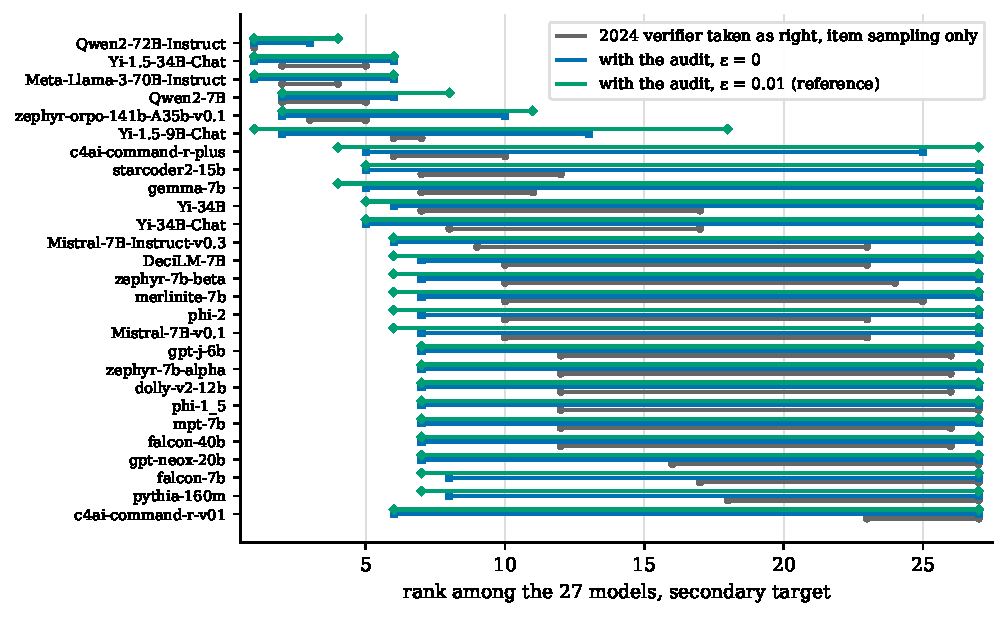
\includegraphics[width=\textwidth]{figures/f5_rank_intervals_generalising.pdf}
\caption{Rank intervals for the secondary target, which also allows for the items being a
sample of possible questions, holding for all orderings at once at an asymptotic level. Grey takes
the 2024 verifier as correct and allows only for item sampling. Without pooling across models (not
drawn), every model's interval spans all \NumModels{} ranks. Compare Figure~\ref{fig:ranks}, which
is the primary target on these items.}
\label{fig:ranks-general}
\end{figure}

The pairing matters separately from the distributional question. An unpaired term, built
from each model's marginal accuracy under one verifier, is kept only to reproduce the
regression anchor of Appendix~\ref{app:tests}; it certifies
\CertSamplingLegacy{} orderings. It is not used, because two models answering the same items
differ on far fewer of them than their marginal accuracies suggest, and a term that ignores
the pairing throws that away.

\subsection{What the coverage simulation does}

The simulation runs \SimScenarios{} scenarios at \SimReplicates{} replicates each, at the full
scale of the roster. It checks whether the guarantee is attained and how it degrades; it is not
a proof.

The frame is the full set of real responses, with the real cell structure and the real audit allocation, so
that the strata, their sizes and their sampling rates are the ones the paper actually uses.
What must be invented is the reader verdict on unaudited responses, and it is invented in two
deliberately different ways.

In the first, each concordant sub-population is given a number of errors that makes the
realised error fractions span an interval of width exactly $\varepsilon_{\mathrm{true}}$, so
that Assumption~\ref{ass:h} holds exactly as a statement about finite populations. This is the
validity check: the procedure is analysed at the same $\varepsilon$, and no certified claim
should be wrong.

In the second, concordant errors are drawn independently with a small propensity that is the
same for every model. No model differs from any other in expectation, which is the most
favourable situation pooling could hope for, and yet the realised fractions differ by chance,
so $H(0)$ fails as a statement about the finite populations that actually exist. This is a
diagnostic rather than a validity check, and it is the one that produced the paper's reason
for not reporting $\varepsilon = 0$ as a result.

Discordant cells are given independent per-model rates drawn uniformly, which is the worst
case the analysis is built for and the reason those cells enter at $[0,1]$ when unaudited.
Items are resampled from the frame with replacement and paired across models, so the
item-sampling term has something real to cover. An audit-only claim is scored against the
difference on the realised items; a combined claim is scored against the superpopulation
expectation. Confusing those two would make the procedure look better than it is, which is why
they are kept apart in the output.

One number bounds what the simulation can resolve. At the nominal level and this many
replicates, the Monte Carlo standard error of a family-wise error rate is \SimMcSeAudit{}, so
a reported rate of zero means below resolution rather than exactly zero, and the scenarios are
compared against nominal with that in mind. Zero failures in \SimReplicates{} replicates is
likewise not a zero error probability: it bounds the family-wise error rate below
\SimZeroFwerUpper{} at \SimZeroFwerConfPct\% confidence, one-sided, so the procedure is
consistent with its stated level and conservative rather than tight.

The second construction is the one that separates the two configurations reported in
Section~\ref{sec:inference}. With equal underlying rates analysed at $\varepsilon = 0$, the
two-verifier analysis exceeds its nominal level and the three-verifier analysis does not, so
exact homogeneity is safe in one configuration and unsafe in the other. Equal underlying rates
do not imply equal realised fractions, so $H(0)$ can fail in the world most favourable to pooling,
which is why the paper does not lead with it.

\section{Sensitivity analyses}
\label{app:sensitivity}

Each analysis in this appendix re-runs the whole pipeline with a single element replaced rather
than recomputing the headline numbers a different way. All but the last row of
Table~\ref{tab:sensitivity} are sensitivity analyses named in our analysis plan; the others it
names are the two-verifier analysis (Section~\ref{sec:results}) and the alternative sampling terms
(Appendix~\ref{app:inference}). The table reports them, with the pooled audit counts each
configuration produces alongside the orderings it certifies, because the counts are what the
certification is downstream of and reporting only the certified number would hide where a
movement came from.

% Generated by scripts/fb_tables_tmlr.py -- do not edit by hand.
\begin{table}[t]
\centering
\caption{Sensitivity analyses. Each row re-runs the whole pipeline with one element of the analysis replaced, and reports the pooled audit counts it produces in the two concordant cells together with the certified orderings, first for the primary target (all orderings at once) and then for the secondary target (one ordering at a time). $^{a}$The pooled interval, in place of Lemma~\ref{lem:kl}. $^{b}$The routine that decides $Y^*$. $^{c}$\textsc{none} and \textsc{contradictory} excluded rather than scored incorrect. $^{d}$Changes the boxed verifier \emph{and} the equivalence routine, so cells move too. $^{e}$A different set of models: its counts are out of a smaller family and are not comparable down the column.}
\label{tab:sensitivity}
\small
\begin{tabular}{lccrrrr}
\toprule
& & & \multicolumn{2}{c}{primary target} & \multicolumn{2}{c}{secondary target} \\
\cmidrule(lr){4-5}\cmidrule(lr){6-7}
analysis & $111$ & $000$ & $\varepsilon=0$ & $\varepsilon=\EpsPrereg$ & $\varepsilon=0$ & $\varepsilon=\EpsPrereg$ \\
\midrule
primary analysis & 142/144 & 0/223 & 208 & 174 & 153 & 131 \\
Clopper--Pearson interval$^{a}$ & 142/144 & 0/223 & 209 & 174 & 155 & 131 \\
Math-Verify equivalence$^{b}$ & 141/144 & 1/223 & 206 & 172 & 143 & 128 \\
indeterminates dropped$^{c}$ & 142/144 & 0/186 & 207 & 174 & 152 & 130 \\
string semantics$^{d}$ & 141/142 & 0/223 & 196 & 168 & 141 & 127 \\
seventeen-model subset$^{e}$ & 142/143 & 0/145 & 99 & 89 & 76 & 68 \\
\bottomrule
\end{tabular}
\end{table}


Four features of the table matter.

The primary result is stable. On these items at the reference tolerance, every alternative
that keeps the verifiers fixed lands within a few orderings of \CertFixedPrereg{}. The choice of
interval makes no difference there at all: Clopper--Pearson, which is tighter but exact only
under assumptions this design does not satisfy, also certifies \SensCpFixed{}. The headline does
not depend on having used the conservative interval, so the conservative one is used because it
is the valid one here, not because the result needs it.

The secondary result moves more, and mostly for one reason. Judging the reader's transcription
with Math-Verify costs the primary target a handful of orderings and the secondary target many
more;
Appendix~\ref{sec:sensitivity} explains why the same labels matter so differently to the two.

The string-semantics row moves both targets furthest, but it changes a verifier as well as the
equivalence routine, so it is not a clean test of either.

The last row is a different question from the others. It restricts the roster to a
seventeen-model subset, so its counts are out of \NumOrderingsSeventeen{} orderings rather than
\NumOrderings{} and cannot be compared down the column. It is in the table because it is the
configuration the regression anchor of Appendix~\ref{app:tests} reproduces.

What none of these rows do is vary Assumption~\ref{ass:h}. They vary the analysis applied to
a fixed assumption. The assumption itself is varied by the $\varepsilon$ curve of
Figure~\ref{fig:eps} and summarised per ordering by the breakdown value, and that is the
sensitivity analysis the paper is actually built around. The rows here answer the narrower
question of whether a defensible alternative choice inside the pipeline would have produced a
different story, and none of them does.

\section{Sensitivity to the equivalence routine and to indeterminate answers}
\label{sec:sensitivity}

Section~\ref{sec:data} defines the reader verdict in two steps, and only the first is human. A
labeller transcribes the final answer a response commits to, and an equivalence routine then
compares that transcription with the benchmark's gold answer; $Y^*$ is whatever the routine
returns. The routine is a choice, and since this paper is about scoring choices that go
unreported, ours is reported here.

The primary analysis uses the benchmark harness's own routine, the same symbolic comparison the
leaderboard applies to its gold answers. We use it because the question is whether a response
would have been credited had a reader, rather than an extraction rule, decided what it says, and
holding the equivalence step at the benchmark's own routine isolates the extraction step, which
is the thing under study. It is not necessarily the best routine available.

\paragraph{A different equivalence routine.}
Deciding $Y^*$ with Math-Verify instead credits \SensMvCorrectRejectAll{} audited response in
the cell where no verifier credits, against \AuditCorrectRejectAll{} under the harness routine,
and \SensMvCorrectAgreeAll{} of \AuditNAgreeAll{} in the cell where all three credit, against
\AuditCorrectAgreeAll{}. Both differences push the bounds the same way. On these items the
certified count moves from \CertFixedEpsZero{} to \SensMvFixedEpsZero{} at $\varepsilon = 0$,
and from \CertFixedPrereg{} to \SensMvFixed{} at the reference tolerance. For the secondary
target it moves from \CertEpsZero{} to \SensMvCombined{} at
$\varepsilon = 0$, one ordering at a time.

The same two labels matter very differently to the two targets, and the reason shows where the
pipeline is fragile. The cell where no verifier credits holds \CellRejectAll{} responses, and
one audited response with reader verdict $1$ raises the upper end of its interval substantially. In the identified range of a pairwise difference, that
interval enters multiplied by the \emph{difference} between the two models' shares of the cell,
which is usually small, because most of every model's responses land there; so the primary
target barely moves. In the sampling term of the secondary target, the same interval enters each model's own
bound on its disagreement with a verifier, multiplied by that model's \emph{own} share, which is
close to one, and the two models' bounds add. That is where most of the secondary target's
movement comes from. The equivalence routine is therefore a minor choice for the primary claim
and a consequential one for the secondary claim.

\paragraph{String comparison.}
The third row of the same family is reported in Table~\ref{tab:sensitivity} and should be read
with care, because it is not a one-factor change. The boxed verifier and the equivalence routine
share a normalisation and comparison implementation, so switching to string comparison
changes which cell a response falls into as well as how its transcription is judged. The
label counts move accordingly: the cell where all three verifiers credit holds
\SensStringNAgreeAll{} audited responses rather than \AuditNAgreeAll{}. On these items at the
reference tolerance certification falls to \SensStringFixed{}; for the secondary target at
$\varepsilon = 0$ it falls to \SensStringCombined{}. We report the row because string
comparison is what the defective
verifier of Section~\ref{sec:data} actually computed, and we do not attribute the movement to
the equivalence routine alone.

\paragraph{Responses with no answer, and responses with two.}
A labeller who finds no final answer records \textsc{none}, and one who finds two answers both
presented as final records \textsc{contradictory}. The primary analysis counts both as
incorrect. The alternative is to drop them, which reduces the audited labels in the cell where
no verifier credits from \AuditNRejectAll{} to \SensDropNRejectAll{}. On these items at the
reference tolerance the certified count stays at \SensDropFixed{}; for the secondary target
at $\varepsilon = 0$ it moves from \CertEpsZero{} to \SensDropCombined{}.

The two agree closely for a mechanical reason.
Dropping the indeterminates removes labels without removing any credited response, so the
numerator stays at its floor while the denominator shrinks; the interval widens slightly and
nothing else moves. The choice would matter more in a cell where indeterminate responses were
a large share of the credited ones, and the design does not guarantee that they never are.

The reason the primary analysis counts them as incorrect is not statistical convenience. Every
verifier in the pipeline scores a response with no extractable final answer as zero, and the
comparison the paper is making is against what the leaderboard reports. Dropping such
responses would compare against a quantity no leaderboard computes, so Section~\ref{sec:data}
makes this choice part of the definition of the reader verdict.

\paragraph{A normalisation rule that edits gold answers.}
The harness normaliser deletes every occurrence of the letters ``ft'' (feet), including inside
LaTeX commands, so \texttt{\textbackslash infty} becomes \texttt{\textbackslash iny} and
\texttt{\textbackslash left} becomes \texttt{\textbackslash le}, and the harness applied it to the
gold answers when it built the dataset; a public discussion of the leaderboard's archive reports
the resulting damage \citep{oll2026discussion}. Normalising each reference solution's boxed answer
with and without the rule, we find \GoldFtItems{} affected items, the number the discussion
reports, and on each the stored answer is the damaged one. The rule is also applied to every transcription, so the reader verdict
compares like with like, but we checked rather than assumed: \GoldFtLabels{} audited labels fall on
these items, \GoldFtConcordant{} of them in a concordant cell, and recomputing their reader verdicts
without the rule changes \GoldFtChanged{} of them. Every certified count is therefore unchanged.

\paragraph{What none of this settles.}
Every row above holds the benchmark's gold answers fixed. An error in a gold answer propagates
identically through the primary analysis and through all of its alternatives, and no
sensitivity analysis run inside the pipeline can detect it. It is the largest thing this design
does not check (Section~\ref{sec:limitations}).

\section{Data, verifiers, and the human audit in detail}
\label{app:data}

\paragraph{How the roster came about.}
By the maintainers' count, the February 2025 re-scoring covered all \BoardModelsRescored{} models
submitted to the leaderboard up to then \citep{kydlicek2025fixing}. An earlier study catalogued all \RosterCatalogued{} of the
leaderboard's per-model result repositories, ranked them by download count, and kept the top
\RosterSelected{} subject to at most \RosterMaxPerOrg{} per organisation, under a rule written
down before any re-scoring; the cap spread the selection over \RosterOrgs{} organisations. A
download sweep over those models was interrupted, and the \RosterScored{} whose downloads
completed were scored. The 400-item audit drew its items from those, and the
roster is the \NumModels{} that received at least one audited item. Every roster model lies
within the first \RosterDeepestRank{} of the download ranking. Against the leaderboard's final
public table, dated \BoardFinalTableDate{}, which lists \BoardModelsFinal{} models with a MATH-Hard
score because submissions continued after the re-scoring,
\RosterBottomQuartile{} of the \NumModels{} fall in the bottom quartile of displayed accuracy
and \RosterTopQuartile{} in the top. The record behind each count is released with its
checksums. A prespecified rule covered missing responses before the data were assembled, and it
did not fire.

\paragraph{The verifiers' provenance.}
The maintainers described the 2024 verifier as unable to extract answers written
in boxed notation and reported that the re-scoring reordered the top of the board
\citep{kydlicek2025fixing}. From the re-scoring on, the leaderboard displayed scores from one
verifier and published item-level verdicts from another. Table~\ref{tab:provenance} gives the
version, a checksum and the check behind every source the analysis rests on, including the
re-execution that reproduces all \EmReexecItems{} published verdicts.

% Generated by scripts/fb_provenance_table.py -- do not edit by hand.
\begin{table}[t]
\centering
\caption{Provenance of every source the analysis rests on. Hashes are the first twelve hexadecimal digits of the sha256 of the file in the release, with line endings normalised; a dash marks an upstream artefact identified by its pinned version instead. Verifier environment: sympy 1.13.1, latex2sympy2\_extended 1.11.0.}
\label{tab:provenance}
\small
\begin{tabular}{p{0.16\textwidth}p{0.3\textwidth}lp{0.3\textwidth}}
\toprule
artefact & version & hash & check \\
\midrule
published responses & 27 per-model result repositories, 189 subject files; revision of each file recorded in the release & \texttt{--} & sample files unmodified since 2024 in 27 of 27 models \\
2024 verifier & lm-evaluation-harness \texttt{3c8db1bb7b} & \texttt{59604119822c} & re-execution reproduces 35{,}748 of 35{,}748 published verdicts \\
Math-Verify & math-verify 0.9.0 via lm-evaluation-harness \texttt{61ee867816} & \texttt{--} & reproduces the re-scored aggregate in 168 of 175 model-subject combinations \\
boxed verifier & lm-evaluation-harness helpers, in the released code & \texttt{ac7865eec34c} & brute-force and printed-formula tests (Appendix~\ref{app:tests}) \\
xFinder & \texttt{IAAR-Shanghai/\allowbreak xFinder-qwen1505} & \texttt{--} & extractions judged by the equivalence routine \\
scores before re-scoring & \texttt{open-llm-leaderboard/\allowbreak results} at \texttt{c6b22601e3} & \texttt{--} & last revision before February 2025 \\
scores after re-scoring & \texttt{open-llm-leaderboard/\allowbreak contents} at \texttt{9c09a7cae4} & \texttt{--} & final revision of the public table \\
all verifier verdicts & released verdict file & \texttt{878751536bfd} & regenerated by the released pipeline \\
\bottomrule
\end{tabular}
\end{table}


% Generated by scripts/fb_tables_tmlr.py -- do not edit by hand.
\begin{table}[t]
\centering
\caption{What the three verifiers share and where they differ. All three rest on the same symbolic algebra library, and the 2024 and boxed verifiers also share the harness's normalisation and the dataset's gold-answer field. Their agreement is informative because their extraction rules and parsers differ, not because they are independent.}
\label{tab:shared}
\begin{tabular}{llll}
\toprule
step & 2024 verifier & boxed verifier & Math-Verify \\
\midrule
answer extraction & sentence pattern & last boxed expression & LaTeX and expression parse \\
normalisation & harness routine & harness routine & latex2sympy2 \\
equivalence & sympy & string, then sympy & Math-Verify \\
gold answer & dataset field & dataset field & parsed from the solution \\
\bottomrule
\end{tabular}
\end{table}


\paragraph{The fourth verifier and its sixteen cells.}
xFinder reads each response and returns an answer or an abstention. An extraction that is empty
or reads ``no valid answer'' (ignoring case, brackets and parentheses) is an abstention and
receives verdict $0$, as does an extraction whose comparison with the gold answer is stopped after
sixty seconds; every other extraction is judged by the equivalence routine that decides the reader
verdict. Appending xFinder's verdict to the three-verifier string gives sixteen cells, of which
\KFourCellsOccupied{} are occupied. The concordant cells are $0000$ and $1111$, and
Assumption~\ref{ass:h} applies to them; the other fourteen are discordant and enter each model's
range at $[0,1]$, as the three-verifier discordant cells do. Every audited response in a three-verifier concordant cell stays concordant
(\KFourAuditNAgreeAll{} labels in $1111$, \KFourAuditNRejectAll{} in $0000$), so the pooled
intervals are unchanged, and the four-verifier count moves only because \KFourMovedFromConcordant{}
responses leave the concordant cells where xFinder disagrees with the other three. The primary
arm uses the system prompt the extractor was fine-tuned with; the other uses its shipped
default.

\paragraph{The defect in our own verifier.}
While tracing where each verdict came from, we found that the boxed verifier had been silently
degraded. Its symbolic comparison guards itself with a timer that exists only on Unix; on Windows
the guard raised an exception, a broad error handler swallowed it, and every comparison returned
``not equivalent'', so every verdict was in effect a string comparison. Correcting it changes the
number of responses on which it disagrees with the 2024 verifier, on a seventeen-model subset kept
as a regression anchor, from \DisagreeSbEmSeventeenString{} to \DisagreeSbEmSeventeen{}. All
results use the corrected verifier. Correcting it also changes the secondary-target certified count on the
seventeen-model regression anchor (Appendix~\ref{app:tests}), one ordering at a time, from
\AnchorStringCombined{} to \AnchorSympyCombined{}. The anchor is the only configuration in which
both versions can be computed on the same labels.

\paragraph{The 400-item audit's discordant labels.}
Some of the 400-item audit's labels land in a discordant cell: \AuditDiscLabels{} of them, all in
one cell, spread over \AuditDiscModels{} models at a median of \AuditDiscMedianPerModel{} per
model. A discordant cell enters the identified range only through a per-model interval, and the
analysis takes those intervals only from labels drawn by model and cell, which these are not. They
therefore appear in Table~\ref{tab:cells} and Figure~\ref{fig:cells} but not in the certified
counts.

\begin{figure}[t]
\centering
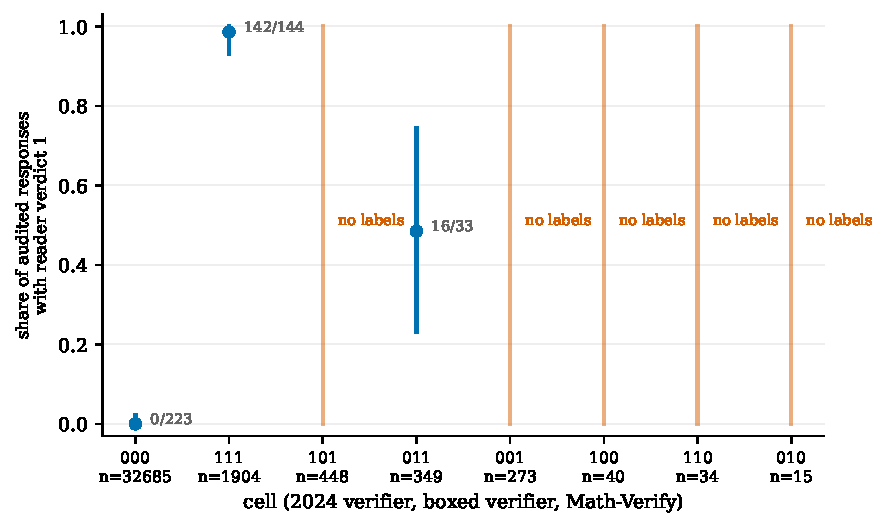
\includegraphics[width=\cellfig]{figures/f3_correctness_by_cell.pdf}
\caption{Share of audited responses in each cell with reader verdict $1$, that is, whose
transcribed answer the benchmark's equivalence routine accepts. Intervals are from
Lemma~\ref{lem:kl}. Five cells carry no labels in the 400-item audit and are bounded only by
$[0,1]$; the labelled discordant cell is shown for description
and does not enter the certification.}
\label{fig:cells}
\end{figure}

\paragraph{How reliable the 400-item audit's labels are.}
The author labelled all 400 items. A second labeller labelled an overlap of \LabTwoN{} of them
and a third a nested overlap of \LabThreeN{}, with both overlaps drawn before any label was seen; each was shown the problem and the response and nothing else. Scoring the
transcribed answers with the equivalence routine, the first and second labellers agree on
\StrOneTwoPct\% of the overlap (Cohen's $\kappa = \StrOneTwoKappa$), the first and third on
\StrOneThreePct\% ($\kappa = \StrOneThreeKappa$), and the second and third on \StrTwoThreePct\%
($\kappa = \StrTwoThreeKappa$). What enters the certification is the reader verdict $Y^*$, and
on it the second labeller agrees with the first on \LabTwoAgree{} of \LabTwoN{} items
($\kappa = \LabTwoKappa$) and the third on \LabThreeAgree{} of \LabThreeN{} ($\kappa =
\LabThreeKappa$). The disagreements are not in the cells that carry the result. In the cell where
no verifier credits there are none (\LabTwoZeroN{} and \LabThreeZeroN{} overlapping labels), and in
the cell where all three credit there are \LabTwoAllDis{} of \LabTwoAllN{} and \LabThreeAllDis{} of
\LabThreeAllN{}; the others fall in discordant cells, which do not enter the counts. Replacing the
first labeller's labels on the overlap by the second labeller's moves the certified count at the
reference tolerance from \CertFixedPrereg{} to \LabSwapTwoPrereg{} (from \CertFixedEpsZero{} to
\LabSwapTwoEpsZero{} at $\varepsilon = 0$), and replacing them by the third's leaves it at
\LabSwapThreePrereg{}. The overlaps are subsets of the 400 items, so this bounds the sensitivity
to the labeller on those subsets only. The audit was labelled in a spreadsheet, so its labels carry no
record of the time spent on each item.

\paragraph{What was fixed, and when.}
Table~\ref{tab:chronology} lists each analysis choice with the document that fixed
it and whether the 400-item audit's labels already existed at the time. Only the audit's design
came before its labels. This study's analysis plan, written for the larger audit before any of that
audit's labels existed, came after the 400-item audit's labels, and so did everything it fixes:
the method of this paper, the tolerance and the sensitivity analyses. The choice of primary target
came later still, after the audit's results for both targets were known. The analysis reported here should therefore be read as
designed with those labels in hand. What protects it from tuning is that every count is reported
as a curve over $\varepsilon$, beside the analysis without pooling, and both targets in full. The
\SuppShort{} holds both documents with their dates.

\begin{table}[h]
\centering
\caption{When each analysis choice was fixed, relative to the 400-item audit's labels.}
\label{tab:chronology}
\small
\begin{tabular}{>{\raggedright\arraybackslash}p{\chronwide}>{\raggedright\arraybackslash}p{\chronmid}>{\raggedright\arraybackslash}p{\chronlast}}
\toprule
choice & fixed in & the audit's labels \\
\midrule
design of the 400-item audit & design document of the earlier study & not yet collected \\
the method: cells, pooled intervals, level allocation & this study's analysis plan and its first four amendments & already existed \\
tolerance $\varepsilon = \EpsPrereg$ and the sensitivity analyses & fourth amendment & already existed \\
fixed-item target as primary & sixth amendment & existed, with results for both targets known \\
larger audit by model and cell, and the discordant census & fourth and sixth amendments & not labelled; no result uses them \\
\bottomrule
\end{tabular}
\end{table}

\section{The roster against the board}
\label{app:board}

Figure~\ref{fig:board-position} places the roster in the distribution of displayed MATH-Hard
accuracy over every model in the leaderboard's final public table (\BoardFinalTableDate{}), and
Figure~\ref{fig:board-shift} plots each traced model's score under the 2024 verifier against its
score under Math-Verify, both read from the same results file. Both use the leaderboard's own
records at fixed revisions; neither involves re-scoring by us. The roster sits low on the board,
and it moved less under the change of verifier than the board did.

\paragraph{Tracing each displayed score.}
The re-scoring rewrote results files in each model's details repository on \BoardRegradeDate{},
changing the MATH-Hard scores and their task version; in every roster file we could compare, the
run's configuration was left unchanged (Table~\ref{tab:provenance}). For each of the \BoardBothModels{} models with a MATH-Hard score both
in the results revision of \BoardPreRescoreDate{} and in the final public table, we listed the
results files in its details repository with the date of the last change to each, read every file
changed on the re-scoring day, and compared its MATH-Hard score with the displayed one, taking the
largest when a model is listed at more than one numerical precision. The displayed score equals the
score of a re-scored file for \BoardAttributable{} models. For \BoardNoRegraded{} models no file was
re-scored, for \BoardMismatch{} the displayed score matches none of the re-scored files, and for
\BoardUnavailable{} the repository could not be read. Over every displayed row of the models we could
read, \BoardStaleRows{} rows match no re-scored file, consistent in kind with a public audit that
reports displayed rows left on the old verifier \citep{oll2026discussion}.

\paragraph{The reversal statistic.}
For \BoardShiftModels{} of the traced models we could also read the re-scored file as it stood before
the re-scoring. Let $a_m$ be model $m$'s MATH-Hard score in that file before the re-scoring and
$b_m$ its score in the same file after it, so that both scores come from one run and one set of
responses. The \BoardShiftModels{} models form \BoardShiftPairs{} unordered pairs $\{i, j\}$. A
pair is \emph{reversed} when $(a_i - a_j)(b_i - b_j) < 0$. The reported share divides the number of
reversed pairs, \BoardShiftReversed{}, by the number of pairs that both scores order strictly,
those with $(a_i - a_j)(b_i - b_j) \neq 0$, of which there are \BoardShiftPairsStrict{}. Pairs tied
under either score (\BoardShiftTiedOld{} under the 2024 score and \BoardShiftTiedNew{} under the
re-scored one, with some overlap) enter neither count; counting them as not reversed instead gives
\BoardShiftReversedAllPct\%. On the roster, \RosterShiftReversed{} of the
\RosterShiftPairsStrict{} strictly ordered pairs reverse. Kendall's $\tau_b$ uses its standard
correction for ties.

A simpler comparison pairs each model's score in the results revision of \BoardPreRescoreDate{}
with its displayed score, and over the \BoardBothModels{} models it gives \BoardSnapshotPct\%. It
mixes runs, though: the earlier revision's score is the same run's score before the re-scoring for
only \BoardSnapshotSameRun{} of the \BoardShiftModels{} same-run models. Restricted to the
\BoardAttributable{} models whose displayed score is a re-scored one, it gives
\BoardAttributablePct\%. The three comparisons agree to within a percentage point.

\paragraph{Were the responses the same?}
The same-run comparison holds the run fixed, and the response files themselves were not rewritten.
For the roster every response file in the model's details repository was last changed in 2024
(Table~\ref{tab:provenance}). For the board we drew \BoardDateSampleN{} of the \BoardBothModels{}
models at random with a fixed seed and read the commit history of every MATH-Hard response file in
each model's details repository; in \BoardDateUnchanged{} of the \BoardDateSampleN{}, every such file
was last changed on or before \BoardPreRescoreDate{}. With no exception in the sample, the share of
the board's models whose response files changed is below \BoardDateUpperPct\% at
\BoardDateConfPct\% confidence (exact, one-sided).

\begin{figure}[htbp]
\centering
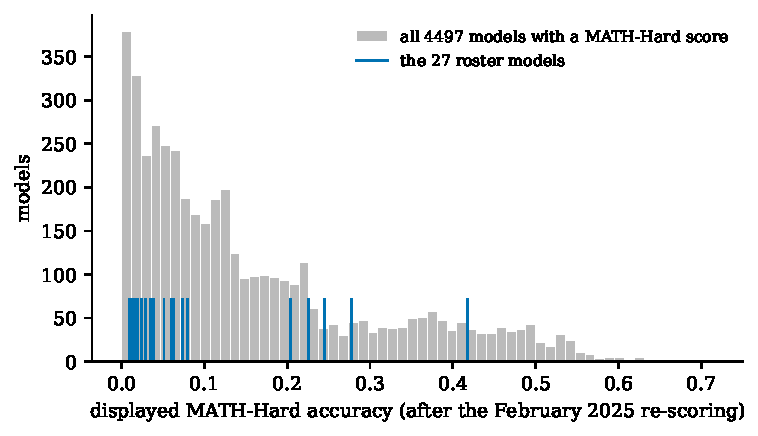
\includegraphics[width=\boardfig]{figures/f6_board_position.pdf}
\caption{Displayed MATH-Hard accuracy after the February 2025 re-scoring, for every model in
the leaderboard's final public table of \BoardFinalTableDate{} (grey), with the roster marked
(blue).}
\label{fig:board-position}
\end{figure}

\begin{figure}[htbp]
\centering
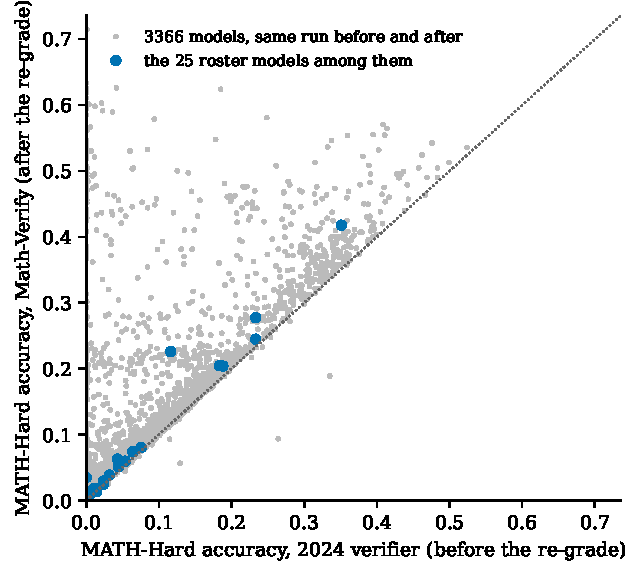
\includegraphics[width=\boardfig]{figures/f8_board_same_run.pdf}
\caption{Each traced model's MATH-Hard accuracy under the 2024 verifier against its accuracy under
Math-Verify, both read from the same results file before and after the re-scoring, for the
\BoardShiftModels{} same-run models; the roster models among them are marked. The responses are
the same on both axes, so points off the diagonal are moved by the verifier alone; the column near
zero on the horizontal axis consists of models whose answers the 2024 verifier could not read.}
\label{fig:board-shift}
\end{figure}

\section{The framework census}
\label{app:frameworks}

% Generated by scripts/fb_tables_tmlr.py -- do not edit by hand.
\begin{table}[t]
\centering
\caption{Scoring configurations that record a failure to extract an answer as an incorrect answer, in four evaluation frameworks at fixed versions. Denominators are different kinds of unit and are not estimates of one common population of tasks. The last column gives, where it was run, the share of sampled units whose behaviour matched their classification, for flagged units and for controls. $^{a}$The version used for the behavioural check; the version used for the classification was not recorded.}
\label{tab:frameworks}
\small
\setlength{\tabcolsep}{3pt}
\begin{tabular}{llrrrl}
\toprule
framework & version & units & flagged & \% & validated \\
\midrule
lm-evaluation-harness & \texttt{f4d4b3de}$^{a}$ & 4{,}524 tasks & 2{,}936 & 64.9 & 93/93 and 100/100 \\
OpenCompass & \texttt{60a28a72} & 1{,}070 configurations & 158 & 14.8 & no \\
lighteval & \texttt{932e1f2f} & 37 metrics & 13 & 35.1 & no \\
simple-evals & \texttt{652c89d0} & 6 string-matching modules & 4 & 66.7 & no \\
\bottomrule
\end{tabular}
\end{table}


Table~\ref{tab:frameworks} summarises the classification of Section~\ref{sec:generality}.
Reading code is not the same as running it, so the classification was validated behaviourally,
for \texttt{lm-evaluation-harness} only; the other three frameworks were classified from their
configurations alone. For a random sample of tasks the declared filter pipeline was rebuilt from the framework's own
classes and run on a well-formed response and on an equivalent response carrying the same
answer in ordinary prose. Of \CensusValidTestable{} testable sampled tasks, all
\CensusValidConfirmed{} behaved as classified, and of \CensusControlN{} control tasks drawn
from the tasks classified as unaffected, all \CensusControlClean{} were confirmed unaffected.

\section{The disagreement taxonomy}
\label{app:gallery}

\paragraph{Template compliance.}
A response is \emph{template compliant} when the 2024 verifier's extraction step finds an answer in
it. That step appends the string ``I hope it is correct.'' to the response and searches the result
(Python's \texttt{re.search}) for the pattern
\texttt{Final Answer: The final answer is(.*?). I hope it is correct.}, whose dots are unescaped
and match any character. The response is compliant when the search succeeds, and the captured
group is the answer the verifier then judges. Compliance is computed for all \NumRows{} responses
with the scoring function recorded in the leaderboard's result files.

\paragraph{The decision tree.}
Every discordant response is classified by the following rules, applied in order; the first rule
that applies decides the class.
\begin{enumerate}
\item \emph{Runtime}: any of the three verifiers timed out or was stopped on the response.
\item \emph{Extraction}: at least one verifier that gave no credit found no answer, meaning that
  the 2024 verifier gave $0$ and the response is not template compliant, the boxed verifier gave
  $0$ and the response contains no \texttt{\textbackslash boxed\{\}}, or Math-Verify gave $0$ and
  could not parse an answer. The sub-class lists every verifier for which this holds (template,
  box, parse, or a combination such as template+box).
\item \emph{Judgement}: otherwise. Every verifier that gave no credit extracted an answer.
\end{enumerate}
The classes are exclusive and cover every discordant response by construction.
Table~\ref{tab:gallery} shows one response of each class, drawn at random with a fixed seed.

% Generated by scripts/fb_extraction_taxonomy.py -- do not edit by hand.
\begin{table}[t]
\centering
\caption{One discordant response per class, drawn at random with a fixed seed rather than chosen, showing its last characters. The cell is the verdict string (2024 verifier, boxed verifier, Math-Verify).}
\label{tab:gallery}
\small
\begin{tabular}{p{0.2\textwidth}cp{0.62\textwidth}}
\toprule
class & cell & end of the response \\
\midrule
extraction: template & 011 & \texttt{\footnotesize fer by that amount.  However, since the order of \$a\$ and \$b\$ does not matter, each pair of polynomials will be counted twice.  Therefore, there are \$\textbackslash{}frac\{12\textbackslash{}cdot2\}\{2\} = \textbackslash{}boxed\{12\}\$ ordered pairs \$(a,b)\$.  The answer is: 12<|im\_start|>user } \\
\addlinespace
extraction: box & 101 & \texttt{\footnotesize ation is accurate, and the answer is well-explained. Good job!   <|im\_start|>\} userNo problem! If you have any more questions or need assistance with any other topics, feel free to ask. I'm here to help!  5The answer is: 5<|im\_start|>\} user} \\
\addlinespace
judgement & 011 & \texttt{\footnotesize g this inequality, we find \$m < -8\$ or \$m > 8\$. Therefore, the possible values of \$m\$ are \$\textbackslash{}boxed\{(-\textbackslash{}infty, -8) \textbackslash{}cup (8, \textbackslash{}infty)\}\$. Final Answer: The final answer is \$(-\textbackslash{}infty, -8) \textbackslash{}cup (8, \textbackslash{}infty)\$. I hope it is correct.  <|im\_start|>user } \\
\addlinespace
\bottomrule
\end{tabular}
\end{table}


\paragraph{By model and by subject.}
Tables~\ref{tab:models} and~\ref{tab:subjects} break the board down further, still without human
labels. The verifiers do not affect every model alike. Template compliance ranges from
\TemplateMinPct\% to \TemplateMaxPct\% of a model's responses, and \RankChangeModels{} of the
\NumModels{} models change rank across the four verifiers. The median change is
\RankSpreadMedian{} place; the largest, \RankSpreadMax{} places, belongs to the model that almost
never writes the template sentence. By Proposition~\ref{prop:oneverifier}, two informative
verifiers whose errors were alike for every model would order every pair the same way, so changes of this kind
show errors that differ across models. By subject, the share of responses in a discordant cell
ranges from \DiscSubjectMinPct\% to \DiscSubjectMaxPct\%, and in every subject most disagreements
are failures to extract, between \ExtrSubjectMinPct\% and \ExtrSubjectMaxPct\% of them, so the
pattern is not confined to one area of the benchmark.

% Generated by scripts/fb_model_subject_table.py -- do not edit by hand.
\begin{table}[t]
\centering
\footnotesize
\caption{Every roster model under each verifier, without human labels; all shares are percentages. Accuracy is the share of the model's responses credited; rank 1 is the highest accuracy among the roster, with ties sharing the best rank, and the spread is the largest minus the smallest of the four ranks. Template is the share of responses in which the 2024 verifier's extraction finds an answer; discordant is the share in a cell where the three verifiers disagree. Rows are in the order of the 2024 verifier.}
\label{tab:models}
\setlength{\tabcolsep}{3pt}
\begin{tabular}{lrrrrcrrr}
\toprule
 & \multicolumn{4}{c}{accuracy} & ranks & & & \\
\cmidrule(lr){2-5}
model & 2024 & boxed & MV & xF & 2024/boxed/MV/xF & spread & template & discordant \\
\midrule
Qwen2-72B-Instruct & 35.1 & 36.6 & 41.7 & 40.6 & 1/1/1/1 & 0 & 83.8 & 8.9 \\
Yi-1.5-34B-Chat & 23.3 & 21.5 & 27.7 & 26.7 & 2/3/2/2 & 1 & 84.8 & 9.2 \\
Meta-Llama-3-70B-Instruct & 23.3 & 24.2 & 24.5 & 24.9 & 2/2/3/3 & 1 & 95.6 & 4.4 \\
Qwen2-7B & 18.8 & 17.7 & 20.4 & 20.4 & 4/5/6/5 & 2 & 94.3 & 5.0 \\
zephyr-orpo-141b-A35b-v0.1 & 18.4 & 14.0 & 20.5 & 20.4 & 5/6/5/5 & 1 & 90.3 & 7.9 \\
Yi-1.5-9B-Chat & 11.6 & 19.6 & 22.6 & 22.2 & 6/4/4/4 & 2 & 45.2 & 12.0 \\
c4ai-command-r-plus & 7.6 & 7.3 & 8.0 & 8.5 & 7/7/7/7 & 0 & 92.4 & 2.3 \\
gemma-7b & 6.4 & 5.6 & 7.5 & 7.4 & 8/8/8/8 & 0 & 75.7 & 3.2 \\
starcoder2-15b & 5.4 & 5.1 & 6.0 & 6.0 & 9/9/10/9 & 1 & 73.3 & 1.7 \\
Yi-34B & 4.5 & 2.7 & 5.1 & 5.1 & 10/11/11/11 & 1 & 69.0 & 3.2 \\
Yi-34B-Chat & 4.3 & 1.7 & 6.3 & 6.0 & 11/16/9/9 & 7 & 55.2 & 5.1 \\
Mistral-7B-Instruct-v0.3 & 3.2 & 2.3 & 3.9 & 3.7 & 12/12/12/12 & 0 & 84.9 & 2.2 \\
Mistral-7B-v0.1 & 2.5 & 1.6 & 2.9 & 2.7 & 13/17/14/14 & 4 & 64.8 & 1.6 \\
DeciLM-7B & 2.4 & 1.9 & 2.8 & 2.6 & 14/13/17/16 & 4 & 65.7 & 1.2 \\
zephyr-7b-beta & 2.4 & 1.8 & 2.9 & 2.6 & 14/15/15/16 & 2 & 83.2 & 1.4 \\
phi-2 & 2.4 & 1.2 & 2.9 & 2.7 & 14/18/15/14 & 4 & 76.6 & 2.2 \\
merlinite-7b & 2.3 & 1.9 & 2.4 & 2.5 & 17/13/18/18 & 5 & 94.4 & 1.1 \\
zephyr-7b-alpha & 1.5 & 0.9 & 2.0 & 1.7 & 18/19/19/19 & 1 & 67.1 & 1.2 \\
dolly-v2-12b & 1.4 & 0.5 & 1.4 & 1.6 & 19/22/24/21 & 5 & 85.8 & 1.1 \\
falcon-40b & 1.4 & 0.8 & 1.8 & 1.7 & 20/20/20/19 & 1 & 65.0 & 1.1 \\
mpt-7b & 1.3 & 0.8 & 1.6 & 1.4 & 21/21/22/22 & 1 & 49.8 & 1.0 \\
gpt-j-6b & 1.2 & 0.5 & 1.4 & 1.4 & 22/23/23/23 & 1 & 42.4 & 1.4 \\
phi-1\_5 & 1.1 & 0.2 & 1.7 & 1.2 & 23/24/21/24 & 3 & 42.1 & 2.0 \\
gpt-neox-20b & 0.6 & 0.2 & 1.4 & 0.9 & 24/26/24/25 & 2 & 39.4 & 1.4 \\
falcon-7b & 0.5 & 0.2 & 1.0 & 0.7 & 25/24/26/26 & 2 & 35.7 & 0.9 \\
pythia-160m & 0.2 & 0.0 & 1.0 & 0.6 & 26/27/26/27 & 1 & 10.8 & 1.0 \\
c4ai-command-r-v01 & 0.0 & 3.2 & 3.5 & 3.5 & 27/10/13/13 & 17 & 0.1 & 3.8 \\
\bottomrule
\end{tabular}
\end{table}

% Generated by scripts/fb_model_subject_table.py -- do not edit by hand.
\begin{table}[t]
\centering
\footnotesize
\caption{The seven MATH-Hard subjects, over all roster responses, without human labels; shares are percentages. Columns as in Table~\ref{tab:models}; extraction is the share of the subject's discordant responses whose disagreement is a failure to extract an answer (Table~\ref{tab:taxonomy}).}
\label{tab:subjects}
\setlength{\tabcolsep}{4pt}
\begin{tabular}{lrrrrrrrr}
\toprule
 & & \multicolumn{4}{c}{accuracy} & & & \\
\cmidrule(lr){3-6}
subject & responses & 2024 & boxed & MV & xF & template & discordant & extraction \\
\midrule
algebra & 8{,}289 & 11.0 & 11.5 & 14.7 & 14.1 & 69.4 & 5.7 & 67.9 \\
intermediate algebra & 7{,}560 & 1.9 & 1.9 & 2.6 & 2.4 & 53.3 & 1.3 & 80.2 \\
prealgebra & 5{,}211 & 13.5 & 11.5 & 15.4 & 15.3 & 75.9 & 5.5 & 88.4 \\
number theory & 4{,}158 & 6.6 & 5.7 & 7.3 & 7.1 & 65.0 & 1.9 & 93.8 \\
precalculus & 3{,}645 & 2.6 & 2.7 & 2.8 & 3.5 & 52.9 & 2.7 & 61.2 \\
geometry & 3{,}564 & 2.8 & 3.0 & 4.0 & 3.6 & 70.5 & 1.7 & 69.4 \\
counting and probability & 3{,}321 & 5.7 & 4.9 & 6.4 & 6.3 & 75.8 & 2.0 & 95.5 \\
\bottomrule
\end{tabular}
\end{table}

\clearpage

\section{Related work in detail}
\label{app:related}

This appendix continues Section~\ref{sec:related} with the comparisons that bear on the design
rather than on the question.

\paragraph{Partial identification with model-generated labels.}
\citet{chen2026partial} study the prevalence of a latent binary attribute when the evidence is a
panel of model reports whose errors may be arbitrarily dependent given the truth. They show that
the prevalence is completely unidentified without restrictions that separate the latent
components, and that weak stochastic-ordering restrictions do not help; identifying power comes
from externally calibrated scores and events, such as reporter accuracy measured on a validation
sample, which they illustrate with a toxicity task that has expert-adjudicated labels. The human
audit in our design plays the role of such a calibration sample. We differ in the target, which
is the difference between models and so an ordering rather than a level; in stratifying by the
agreement of several verifiers, so that the calibration assumption is confined to the cells where
they agree; in carrying the assumption as a parameter $\varepsilon$ with a breakdown value for
each conclusion; and in intervals that are valid under sampling without replacement.

\paragraph{Uncertainty in rankings.}
Rank confidence intervals for language-model leaderboards already exist, built by aggregating
pairwise tests, and recent work examines where their uncertainty comes from on a knowledge
benchmark, in particular variability across subjects \citep{neuhof2026ranking}. That uncertainty is
about which items were asked. The uncertainty here is about how each item was scored, and it
does not shrink as items are added; the secondary analysis of this paper combines the two.

\paragraph{Reporting how far an assumption can be pushed.}
Assumption~\ref{ass:h} is not testable at this budget in any strong sense, so the useful thing to
report is how much of it a conclusion needs. Design sensitivity describes a finding by the
magnitude of unmeasured bias that would be required to explain it away, and compares designs by
how much bias they can tolerate \citep{rosenbaum2004design}; $\varepsilon^{*}_{jk}$ is the amount
of cross-model heterogeneity it would take to overturn $j \succ k$. The analogy also sets the
reporting standard followed here, which attaches the sensitivity parameter to each conclusion as
a number instead of leaving it as a caveat in a discussion section.

\paragraph{Two-phase sampling, verification bias, and raters without a gold standard.}
Two-phase sampling, in which a large first-phase sample is measured cheaply and a small second
phase accurately, goes back to \citet{neyman1938contribution}, and the binomial case with
misclassification, where a fallible classifier is calibrated against a subsample scored by an
infallible one, is \citeauthor{tenenbein1970double}'s double sampling scheme
\citep{tenenbein1970double}. When the subsample is chosen by the fallible classifier's own
verdict, the problem is verification bias, and corrections for it are standard in diagnostic
testing \citep{begg1983assessment}; confidence limits that propagate uncertainty in the
estimated error rates into the corrected prevalence are also available \citep{lang2014confidence}.
Two features of our setting break the classical correction. The reader verdict is observed on a
sample stratified by the agreement pattern of several verifiers rather than by one verifier's
verdict, and the error rates are not assumed common across the populations being compared, which
is the assumption Proposition~\ref{prop:oneverifier} shows to be fatal to the question.

Estimating error rates from several imperfect tests without a gold standard is classical
\citep{hui1980estimating}, as is estimating observer error rates from repeated labels
\citep{dawid1979maximum}. Those methods identify rates by assuming the raters err independently
given the truth. We do not assume that, and Section~\ref{sec:data} reports what the three
verifiers share. Instead of identifying the rates through an independence assumption, we obtain
partial identification from agreement stratification and accept wider intervals.

\paragraph{Where to spend a label budget.}
Deciding how many labels each stratum receives is a stratified sampling problem, and the
classical answer optimises the variance of an estimated mean \citep{neyman1934stratified}, with
unequal selection probabilities handled by the standard weighting
\citep{horvitz1952generalization} and the finite-population corrections used here taken from the
standard texts \citep{cochran1977sampling, kish1965survey}. Adaptive versions that learn the
within-stratum variances while sampling are recent \citep{morikawa2026tsneyman}. An audit designed
for certification faces a different problem. A label can narrow an identified range or test the
assumption on which every certified ordering depends, and the two uses are not commensurable, so
no single variance criterion allocates between them.
